\documentclass{article}
\usepackage{graphicx}
\usepackage{subcaption}
\usepackage{listings}
\usepackage{color}
\usepackage{hyperref}

\renewcommand\lstlistingname{Quelltext} % Change language of section name

\lstset{ % General setup for the package
	language=Perl,
	basicstyle=\small\sffamily,
	numbers=left,
 	numberstyle=\tiny,
	frame=tb,
	tabsize=4,
	columns=fixed,
	showstringspaces=false,
	showtabs=false,
	keepspaces,
	commentstyle=\color{red},
	keywordstyle=\color{blue}
}

\title{Rapport de stage}
\date{2019-06-01 2019-08-01}
\author{Lecleire Sebastien}
\pagenumbering{arabic}
\begin{document}

\begin{titlepage}
	\centering
	
\includegraphics[width=0.4\textwidth]{irif_horizontal}
	
\includegraphics[width=0.4\textwidth]{Logo80ANS_OR}\par\vspace{1cm}
	
\includegraphics[width=0.4\textwidth]{logop7}
	
\includegraphics[width=0.4\textwidth]{Universite_Paris_logo_horizontal}\par\vspace{1cm}
	{\scshape\LARGE Université Paris Diderot \par}
	\vspace{1cm}
	{\scshape\Large Rapport de Stage\par}
	\vspace{1.5cm}
	{\Large\itshape Sébastien Lecleire\par}
	\vfill
	supervisé par\par
	Yann \textsc{Régis-Gianas}

	\vfill
\end{titlepage}


\newpage

\tableofcontents
\newpage

\section{Remerciements}
Je tiens à remercier toutes les personnes qui ont contribué au succès de mon stage et qui m'ont aidé lors de la rédaction de ce rapport.

Tout d'abord, j'adresse mes remerciements à mon professeur, Mr Joseph X de l'Université Y qui m'a beaucoup aidé dans ma recherche de stage et m'a permis de postuler dans cette entreprise. Son écoute et ses conseils m'ont permis de cibler mes candidatures, et de trouver ce stage qui était en totale adéquation avec mes attentes.

Je tiens à remercier vivement mon maitre de stage, Mr Gabriel X, responsable du service Y au sein de l'entreprise F, pour son accueil, le temps passé ensemble et le partage de son expertise au quotidien. Grâce aussi à sa confiance j'ai pu m'accomplir totalement dans mes missions. Il fut d'une aide précieuse dans les moments les plus délicats.

Je remercie également toute l'équipe E pour leur accueil, leur esprit d'équipe et en particulier Mr DDDD, qui m'a beaucoup aidé à comprendre les problématiques d'achats sécurisés...

Enfin, je tiens à remercier toutes les personnes qui m'ont conseillé et relu lors de la rédaction de ce rapport de stage : ma famille, mon amie Julie B camarade de promotion.


\newpage

\section{Introduction}


En 2060, 90\% des français rouleront dans des véhicules électriques, un chiffre très fort révélé par l'étude "Ma voiture du futur" de xxxx en 201X, et qui en dit long sur les changements futurs dans le domaine de l'automobile.

Dans le cadre de ma Licence XXX à l'Université XXX, j'ai souhaité réaliser mon stage dans une entreprise répondant à ces enjeux du futur en matière de mode de transport et d'écologie... tout en me formant aux métiers de community manager... que j'ai découvert et que ma formation propose comme débouché.... Les missions de xxx et zzz m'ont attiré particulièrement car j'ai un esprit créatif et je souhaitais savoir si ce type de métier pouvait m'intéresser puisque je m'oriente dans ma formation et professionnellement vers le marketing et la communication.
Aussi l'entreprise française RRRRR, créée très récemment en 2014.... s'est fait connaitre avec succès pour ses produits innovants..., j'ai voulu intégrer ses équipes pour pouvoir découvrir leurs méthodes et principes industriels reconnus sur le marché. Nous verrons ainsi au travers de ce rapport la problématique actuelle du secteur : quels sont les freins et les leviers de l'automobile électrique en ville ?

Dans un premier temps nous décrirons l'entreprise et son secteur en insistant sur ses particularités notamment dans le financement international. Puis nous étudierons mes missions, lors de ce stage avant de dresser un bilan de celui-ci.

\newpage

\section{L'IRIF}

\subsection{le secteur d'activité (les concurrents, les besoins des consommateurs)}

\subsection{l'entreprise (son historique, ses forces / faiblesses, son organisation)}

\newpage

\section{Mon stage}

21. 
22. 

\subsection{les missions (responsabilités, tâches à effectuer, dossiers confiés, objectifs)}

\subsection{le bilan
résultats obtenus ( appréciation du maître de stage - productivité ... gestion du temps)
difficultés rencontrées et solutions apportées
enseignements/apports du stage (connaissances - compétences)}

\newpage

\section{A trouver}
Merci !

\subsection{Subsection}

\newpage

\section{Conclusion}

Ce stage a été très enrichissant pour moi car il m’a permis de découvrir dans le détail le secteur du ………, ses acteurs, contraintes… et il m’a permis de participer concrètement à ses enjeux au travers de mes missions variées comme celle du …. que j’ai particulièrement apprécié. Ce stage m’a aussi permis de comprendre que les missions créatives n’étaient pas les plus adaptées pour moi…et je préfère m’orienter vers les métiers de …. qui me conviennent mieux.(Cette partie doit faire le bilan des plus et moins du stage / votre enrichissement pour votre future carrière)


L’entreprise … qui m’a accueilli pendant ce stage fait face à une période charnière…, et je suis très fier d’avoir pu contribuer, participer à cette révolution. L’évolution des usages et l’adaptation de l’entreprise au changement de son environnement….
(Cette partie doit montrer que vous avez su comprendre les enjeux économiques des secteurs de l’entreprise et/ou réponse à la problématique du rapport)


Fort de cette expérience et en réponse à ses enjeux, j’aimerai beaucoup par la suite essayer de m’orienter via un prochain stage, vers le secteur … avec des acteurs de petites tailles, et un important développement d’avenir.
(ouverture …prochaine étape)


\newpage
\section{Tests}
\begin{figure}[h!]
  \centering
  \begin{subfigure}[b]{0.2\linewidth}
    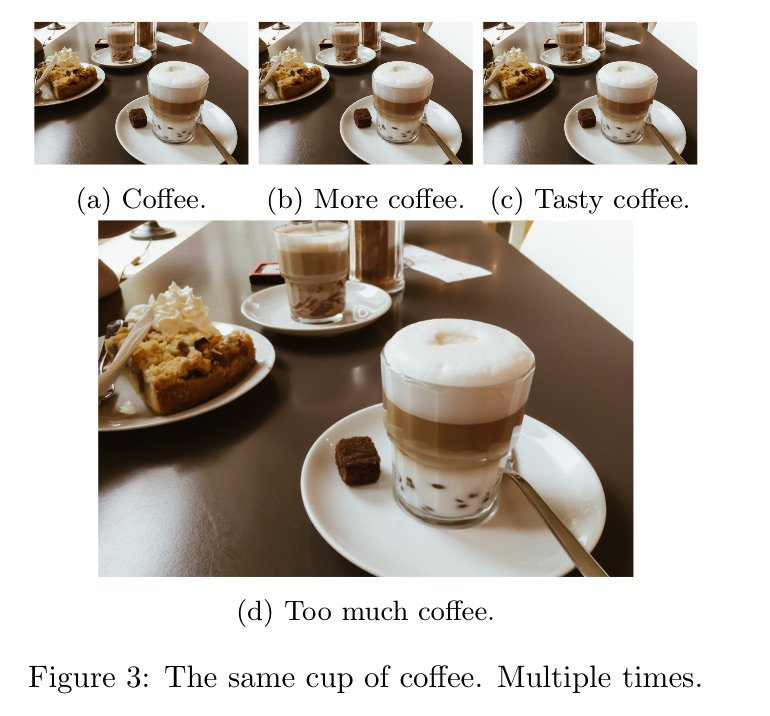
\includegraphics[width=\linewidth]{coffee.jpg}
     \caption{Coffee.}
  \end{subfigure}
  \begin{subfigure}[b]{0.2\linewidth}
    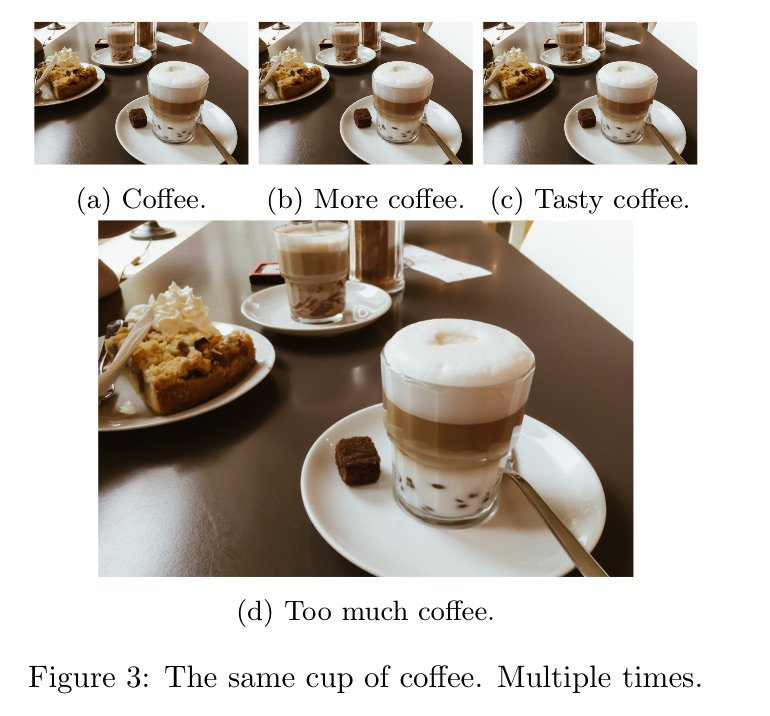
\includegraphics[width=\linewidth]{coffee.jpg}
    \caption{More coffee.}
  \end{subfigure}
  \begin{subfigure}[b]{0.2\linewidth}
    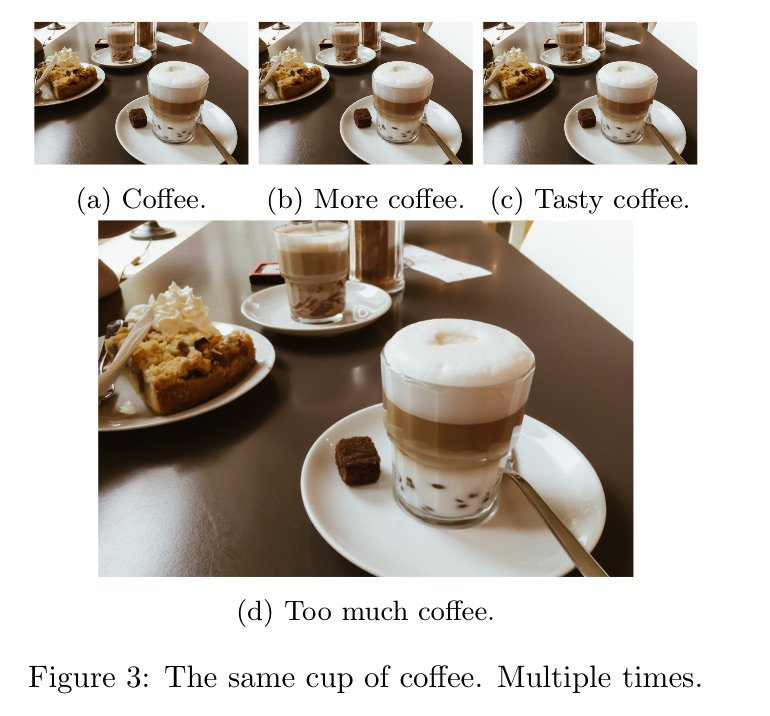
\includegraphics[width=\linewidth]{coffee.jpg}
    \caption{Tasty coffee.}
  \end{subfigure}
  \begin{subfigure}[b]{0.5\linewidth}
    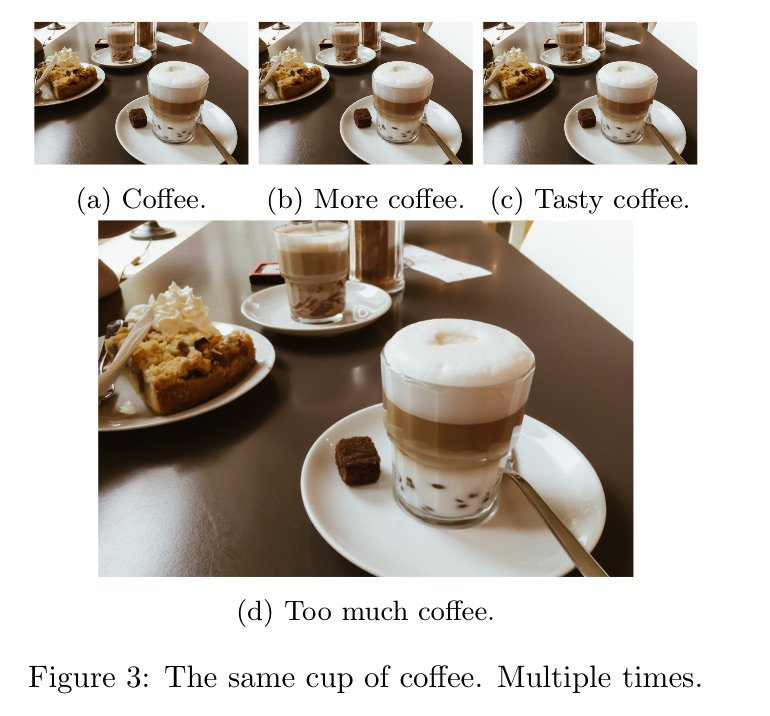
\includegraphics[width=\linewidth]{coffee.jpg}
    \caption{Too much coffee.}
  \end{subfigure}
  \caption{The same cup of coffee. Multiple times.}
  \label{fig:coffee3}
 
\end{figure}

Test of a link : \href{http://www.atec.com}{ici}

Random citation \cite{WEBSITE:1} embeddeed in text.

\begin{lstlisting}
#!/usr/bin/perl
print S(@ARGV);sub S{$r=(@_[0]%4==0&&@_[0]%100!=0)||@_[0]%400=0;}
\end{lstlisting}

\newpage

\bibliography{library}
\bibliographystyle{ieeetr}
\end{document}
